\section[Newton versus Einstein]{\hyperlink{toc}{Newton versus Einstein}}

\subsection{Evidence for electrical neutrality}
Through astronomical observations, we notice that gravitational forces dominate dynamics in the universe on large scales. However, electrostatic forces are much stronger than gravitational. A simple demonstration of this is given by comparing the magnitudes of the gravitational and electrostatic forces between an electron and proton. At a distance $r$, the gravitational force between an electron and proton (in the Newtonian picture) is given by:
\begin{equation}
    \abs{F_g} = \frac{Gm_p m_e}{r^2} = \frac{1}{r^2}(6.67 \times 10^{-11} \si{N.kg^{-2}.m^2})(1.67 \times 10^{-27} \si{kg})(9.11 \times 10^{-31}\si{kg}) = \frac{1.01 \times 10^{-66}}{r^2} \si{N}
\end{equation}
And the elecctrostatic force is given by:
\begin{equation}
    \abs{F_e} = \frac{k e^2}{r^2} = \frac{1}{r^2}(8.99 \times 10^{9} \si{N.C^{-2}.m^2})(1.60 \times 10^{-19} C)^2 = \frac{2.30\times 10^{-28}}{r^2} \si{N}
\end{equation}
Taking the ratio we have:
\begin{equation}
    \abs{\frac{F_e}{F_g}} = \abs{\frac{\frac{2.30\times 10^{-28}}{r^2} \si{N}}{\frac{1.01 \times 10^{-66}}{r^2} \si{N}}} = 2.28 \times 10^{38}
\end{equation}
As we can see from this example, electrostatic forces are much stronger than gravitational (38 orders of magnitude stronger in this case!). Hence if there was a large charge imbalance in the universe, we would observe that electrostatic forces would dominate large-scale dynamics rather than gravitational. This however disagrees with our observations, and we conclude that the universe must be (mostly) electrically neutral.

\subsection{Angular Width on a sphere}
We recall that the metric for a sphere of radius $R$ is given by:
\begin{equation}
    dl^2 = dr^2 + R^2\sin^2\left(\frac{r}{R}\right)d\theta^2
\end{equation}
So we can write the width $dl$ of the object using the above equation. Since $dl \ll R$, we can take the entire width of the object to be located at the same distance $r$ away from us (the observer). In other words, in this limit we have $dr = 0$ and hence the above reduces to:
\begin{equation}
    dl^2 = R^2\sin^2\left(\frac{r}{R}\right)d\theta^2
\end{equation}
Isolating for the angular width of the object, we obtain:
\begin{equation}
    \boxed{d\theta = \frac{dl}{R\sin(\frac{r}{R})}}
\end{equation}
As we take $r \to \pi R$ (i.e. the object is located at the antipode) we have:
\begin{equation}
   \lim_{r \to R\pi} d\theta = \lim_{r \to R\pi} \frac{dl}{R\sin(\frac{r}{R})} = \infty
\end{equation}
as the denominator goes to 0 ($\lim_{r \to R\pi}\sin(\frac{r}{R}) = \sin(\frac{R\pi}{R}) = \sin(\pi) = 0$). The angular width is minimized when the object lies on the equator, where $r = \frac{R\pi}{2}$ and $d\theta = \frac{dl}{R}$, and this angular width increases to infinity as the object approaches the antipode of the sphere. For an object at the antipode, all lines of sight from the observer lead to the object, and it therefore fills the horizon.

\subsection{The Earth isn't flat!}
We choose our coordinate system such that the origin is located in the center of the sphere, and we as the oberver are located at the north pole. The circle drawn on the sphere is at a fixed distance $r$ from us on the north pole, and therefore each point on the sphere is at a fixed polar angle $\theta$. The radius of this circle as measured as an outside observer (not located on the sphere) is $R \sin\theta$.
\begin{figure}[htbp]
    \centering
    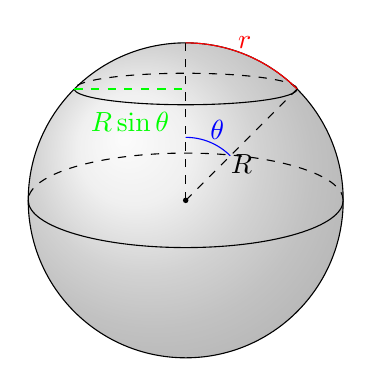
\begin{tikzpicture}
        \shade[ball color = gray!40, opacity = 0.4] (0,0) circle (2cm);
        \draw (0,0) circle (2cm);
        \draw (-2,0) arc (180:360:2 and 0.6);
        \draw[dashed] (2,0) arc (0:180:2 and 0.6);
        \fill[fill=black] (0,0) circle (1pt);
        \draw[dashed] (0,0) -- node[below]{$R$} (1.414,1.414);
        \draw (-1.414, 1.414) arc (180:360:1.414 and 0.2);
        \draw[dashed] (1.414, 1.414) arc (0:180:1.414 and 0.2);
        \draw[dashed] (0, 0) -- (0, 2);
        \draw[blue] (0, 0.8) arc (90:45:0.8);
        \node[blue] at (0.4, 0.9) {$\theta$};
        \draw[red] (0, 2) arc (90:45:2);
        \node[red] at (0.75, 2) {$r$};
        \draw[dashed, green] (-1.414, 1.414) -- (0, 1.414);
        \node[green] at (-0.707, 1) {$R\sin\theta$};
    \end{tikzpicture}
    \caption{Illustration of setup of Problem 3.3}
    \label{fig3.3}
\end{figure}
The circumference of the circle is therefore given by:
\begin{equation}
    C = 2\pi R \sin \theta
\end{equation}
Now, we recall that the arclength $r$ is related to the polar angle and sphere radius by:
\begin{equation}
    r = R\theta.
\end{equation}
So substituing this into the circumference, we obtain:
\begin{equation}\label{circsphere}
    \boxed{C = 2\pi R\sin(\frac{r}{R})}
\end{equation}
which was the claimed formula. For the second part of the question, we consider that for a flat space, the circumference would be measured to be:
\begin{equation}
    C_f = 2\pi r.
\end{equation}
In the limit $r \ll R$, we can Taylor expand the circumference as given in Eq. \eqref{circsphere} to obtain that:
\begin{equation}
    C_s \approx 2\pi R\left(\frac{r}{R} - \frac{r^3}{6R^3}\right) = 2\pi r - \frac{\pi r^3}{3R^2}
\end{equation}
Hence the difference between the circumference measured in Euclidean space versus a sphere would be given by:
\begin{equation}
    \abs{C_f - C_s} \approx \abs{2\pi r - (2\pi r - \frac{\pi r^3}{3R^2})} = \frac{\pi r^3}{3R^2}.
\end{equation}
We can measure distances within an error of $\pm 1\si{m}$, so to convince ourselves that Earth is spherical rather than flat, we require that the circumference differnece be:
\begin{equation}
    \abs{C_f - C_s} > 1\si{m}
\end{equation}
So approximately:
\begin{equation}
    \frac{\pi r^3}{3R^2} > 1 \si{m}
\end{equation}
Rearranging, we have:
\begin{equation}
    r > \sqrt[3]{\frac{3\si{m} R^2}{\pi}}
\end{equation}
And substituing $R = 6400\si{km}$ we get:
\begin{equation}
    \boxed{r > 34\si{km}}
\end{equation}

\subsection{Area Bounds for Equilateral Triangles}
\textbf{Case 1: $\kappa = +1$}. No, we cannot draw an equilateral triangle of arbitrarily large surface area $A$ in this case. A simple counterargument is that a sphere has surface area $4\pi R^2$, so immediately no triangle with area larger than that is possible. For a calculation of the maximum area of a triangle, we require a thoughtful argument. First, recall the equation for the sum of three angles of a triangle of area $A$ on a surface of a sphere of radius $R$:
\begin{equation}
    \alpha + \beta + \gamma  = \pi + \frac{A}{R^2}
\end{equation}
For an equiliateral triangle, $\alpha = \beta = \gamma$, so:
\begin{equation}\label{sphereangles}
    3\alpha = \pi + \frac{A}{R^2}
\end{equation}
WLOG, we can choose our coordinate system that the first point of the triangle is on the north pole, the second point is a distance $r$ from the north pole on the sphere with azimuthal angle $\phi = 0$, and the third point is also a distance $r$ from the north pole on the sphere with azimuthal angle $\phi = \alpha$.

\begin{figure}[htbp]
    \centering
    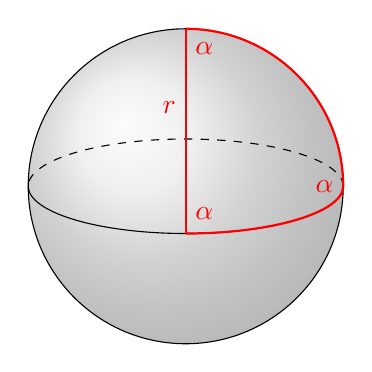
\begin{tikzpicture}
        \shade[ball color = gray!40, opacity = 0.4] (0,0) circle (2cm);
        \draw (0,0) circle (2cm);
        \draw (-2,0) arc (180:360:2 and 0.6);
        \draw[dashed] (2,0) arc (0:180:2 and 0.6);
        \draw[red, thick] (0, 2) arc (90:0:2);
        \draw[red, thick] (0, 2) -- (0, -0.6);
        \draw[red, thick] (0,-0.6) arc (270:360:2 and 0.6);
        \node[red, left] at (0, 1) {$r$};
        \node[red, right] at (0, 1.75) {$\alpha$};
        \node[red, right] at (0, -0.35) {$\alpha$};
        \node[red, left] at (2, 0) {$\alpha$};
    \end{tikzpicture}
    \caption{Illustration of the triangle drawn for the spherical case of Problem 3.4.}
    \label{fig3.4}
\end{figure}

\noindent We now recall the area element on the sphere is given as:
\begin{equation}
    dA = R d\theta \cdot R \sin\theta d\phi = R^2 d\theta d\phi 
\end{equation}
Where $Rd\theta$ is the polar distance and $R\sin\theta d\phi$ is the azimuthal distance. With the setup as described, the area of the triangle may be calculated via integration. We integrate from $0 \leq \theta \leq \frac{r}{R}$ (recalling that $r = R\theta$) and from $0 \leq \phi \leq \alpha$:
\begin{equation}
    A = \iint_{\text{triangle}} dA = R^2 \int_{0}^{r/R} \sin\theta d\theta \int_{0}^{\alpha} d\phi 
\end{equation}
Carrying out these two easy integrals, we obtain:
\begin{equation}
    A = R^2 \left(1 - \cos(\frac{r}{R})\right)\alpha
\end{equation}
Isolating for $\alpha$, we obtain:
\begin{equation}
    \alpha = \frac{A}{R^2\left(1 - \cos(\frac{r}{R})\right)}
\end{equation}
Plugging this into \eqref{sphereangles}, we get:
\begin{equation}
    3\frac{A}{R^2\left(1 - \cos(\frac{r}{R})\right)} = \pi + \frac{A}{R^2}
\end{equation}
Isolating for $A$ we have:
\begin{equation}
    A = \pi R^2 \frac{1 - \cos(\frac{r}{R})}{2 + \cos(\frac{r}{R}) }
\end{equation}
The largest that $r$ can possibly be is when $r = \pi R$ (the base of the triangle lies on the south pole), and so:
\begin{equation}
    \boxed{A_{\text{max}} = \pi R^2 \frac{1 - \cos(\frac{\pi R}{R})}{2 + \cos(\frac{\pi R}{R}) } = \pi R^2 \frac{1 - (-1)}{2 - 1} = 2\pi R^2}
\end{equation}
In other words, the largest an equilateral triangle can be in this case is being half of the sphere!

\noindent \textbf{Case 2: $\kappa = 0$}. We can draw an equilateral triangle of arbitrarily large surface area $A$ in this case. On a flat plane, there is no upper bound to how large you want to draw your shapes!

\noindent \textbf{Case 3: $\kappa = -1$}. No, we cannot draw an equilateral triangle of arbitrarily large surface area $A$ in this case. Consider the equation that gives the sum of three angles of a triangle on a 2-D surface of uniform negative curvature (with radius of curvature $R$):
\begin{equation}
    \alpha + \beta + \gamma = \pi - \frac{A}{R^2}
\end{equation}
For an equilateral triangle, $\alpha = \beta = \gamma$ so:
\begin{equation}
    3\alpha = \pi - \frac{A}{R^2}
\end{equation}
$\alpha$ cannot be negative if we are to have a physical shape, so:
\begin{equation}
    0 \leq \pi - \frac{A}{R^2}
\end{equation}
Rearranging, we obtain an upper bound on the area of an equilateral triangle for a 2-D surface of uniform negative curvature:
\begin{equation}
   A \leq R^2\pi
\end{equation}
Which gives us a maximum:
\begin{equation}
    \boxed{A_{\text{max}} = R^2\pi}
\end{equation}
in this limit, note that the angles of the triangle $\alpha$ approach zero.

\subsection{Equivalent Metrics}
We wish to show the equivalence of the metrics:
\begin{equation}\label{3.29}
    dl^2 = dx^2 + dy^2 + dz^2
\end{equation}
and:
\begin{equation}\label{3.30}
    dl^2 = dr^2 + r^2\left[d\theta^2 + \sin^2\theta d\phi^2\right].
\end{equation}
Making the substitutions $x = r\sin\theta\cos\phi$, $y = r\sin\theta\sin\phi$, and $z = r\cos\theta$ into \eqref{3.29}, we have:
\begin{equation}
    dl^2 = (d(r\sin\theta\cos\phi))^2 + (d(r\sin\theta\sin\phi))^2 + (d(r\cos\theta))^2
\end{equation}
Liberally applying the product and chain rules, we obtain:
\begin{multline}
    dl^2 = (\sin\theta\cos\phi dr + r\cos\theta\cos\phi d\theta - r\sin\theta\sin\phi d\phi)^2
    \\ + (\sin\theta\sin\phi dr + r\cos\theta\sin\phi d\theta + r\sin\theta\cos\phi d\phi)^2
    \\ + (\cos\theta dr - r\sin\theta d\theta)^2
\end{multline}
Now we can expand this expression:
\begin{multline}
    dl^2 = \sin^2\theta \cos^2\phi dr^2 + r^2\cos^2\theta\cos^2\phi d\theta^2 + r^2\sin^2\theta\sin^2\phi d\phi^2
    \\ + 2r\sin\theta\cos\theta\cos^2\phi dr d\theta - 2r\sin^2\theta \sin\phi\cos\phi dr d\phi - 2r^2\sin\theta\cos\theta\sin\phi\cos\phi d\theta d\phi
    \\ + \sin^2\theta\sin^2\phi dr^2 + r^2\cos^2\theta\sin^2\phi d\theta^2 + r^2\sin^2\theta\cos^2\phi d\phi^2
    \\ + 2r\sin\theta\cos\theta\sin^2\phi drd\theta + 2r\sin^2\theta\sin\phi\cos\phi dr d\phi + 2r^2\sin\theta\cos\theta\sin\phi\cos\phi d\theta d\phi
    \\ + \cos^2\theta dr^2 - 2r\sin\theta\cos\theta dr d\theta + r^2\sin^2\theta d\theta^2
\end{multline}
Now grouping like terms, we have:
\begin{multline}
    dl^2 = dr^2\left[\sin^2\theta \cos^2\phi + \sin^2\theta\sin^2\phi + \cos^2\theta\right] + r^2 d\theta^2\left[\cos^2\theta\cos^2\phi + \cos^2\theta\sin^2\phi + \sin^2\theta\right]
    \\ + r^2d\phi^2 \left[\sin^2\theta\sin^2\phi + \sin^2\theta\cos^2\phi\right] + 2r drd\theta \left[\sin\theta\cos\theta\cos^2\phi + \sin\theta\cos\theta\sin^2\phi - \sin\theta\cos\theta\right]
    \\ + 2rdrd\phi \left[-\sin^2\theta \sin\phi\cos\phi + \sin^2\theta\sin\phi\cos\phi\right] + 2r^2d\theta d\phi\left[-\sin\theta\cos\theta\sin\phi\cos\phi + \sin\theta\cos\theta\sin\phi\cos\phi\right]
\end{multline}
We can see the last line of terms all equals to zero (the brackets evaluate to zero, so):
\begin{multline}
    dl^2 = dr^2\left[\sin^2\theta \cos^2\phi + \sin^2\theta\sin^2\phi + \cos^2\theta\right] + r^2 d\theta^2\left[\cos^2\theta\cos^2\phi + \cos^2\theta\sin^2\phi + \sin^2\theta\right]
    \\ + r^2d\phi^2 \left[\sin^2\theta\sin^2\phi + \sin^2\theta\cos^2\phi\right] + 2r drd\theta \left[\sin\theta\cos\theta\cos^2\phi + \sin\theta\cos\theta\sin^2\phi - \sin\theta\cos\theta\right]
\end{multline}
Now redrawing some brackets:
\begin{multline}
    dl^2 = dr^2\left[\sin^2\theta(\cos^2\phi + \sin^2\phi) + \cos^2\theta\right] + r^2 d\theta^2\left[\cos^2\theta(\cos^2\phi + \sin^2\phi) + \sin^2\theta\right]
    \\ + r^2d\phi^2 \left[\sin^2\theta(\sin^2\phi + \cos^2\phi)\right] + 2r drd\theta \left[\sin\theta\cos\theta(\cos^2\phi + \sin^2\phi) - \sin\theta\cos\theta\right]
\end{multline}
Now applying the $\cos^2\phi + \sin^2\phi = 1$ identity to each term:
\begin{equation}
    dl^2 = dr^2\left[\sin^2\theta + \cos^2\theta\right] + r^2 d\theta^2\left[\cos^2\theta + \sin^2\theta\right]
    \\ + r^2d\phi^2 \left[\sin^2\theta \right] + 2r drd\theta \left[\sin\theta\cos\theta - \sin\theta\cos\theta\right]
\end{equation}
The last term vanishes, and to the first two terms we can apply the identity $\cos^2\theta + \sin^2\theta = 1$:
\begin{equation}
    dl^2 = dr^2 + r^2d\theta^2 + r^2\sin^2\theta d\phi^2
\end{equation}
And redrawing some brackets:
\begin{equation}
    dl^2 = dr^2 + r^2\left[d\theta^2 + \sin^2\theta d\phi^2\right]
\end{equation}
We identify this with \eqref{3.30} and hence we conclude.